\begin{figure}[htbp]
\centering
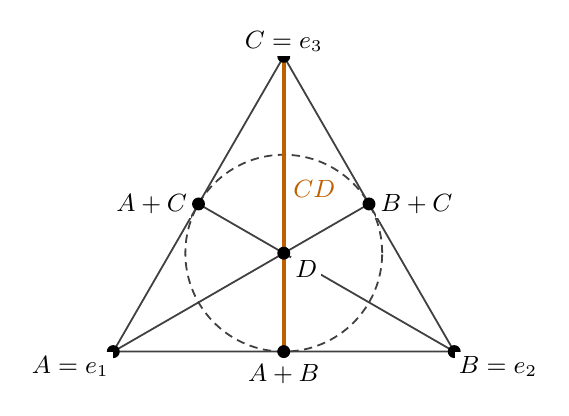
\begin{tikzpicture}[x=1.25cm,y=1.25cm,
  fano edge/.style={draw=black!75,line width=.65pt},
  fano point/.style={circle,fill=black,inner sep=1.65pt},
  fano label/.style={font=\small,fill=white,inner sep=1.5pt}]
  \coordinate (A) at ({-sqrt(3)},-1);
  \coordinate (B) at ({sqrt(3)},-1);
  \coordinate (C) at (0,2);
  \coordinate (D) at (0,0);
  \coordinate (AB) at (0,-1);
  \coordinate (AC) at ({-sqrt(3)/2},.5);
  \coordinate (BC) at ({sqrt(3)/2},.5);
  \draw[fano edge] (A)--(B)--(C)--cycle;
  \draw[fano edge] (A)--(BC) (B)--(AC);
  \draw[fano edge,densely dashed] (D) circle[radius=1];
  \draw[draw=orange!75!black,line width=1.35pt] (C)--(AB);
  \foreach \P in {A,B,C,D,AB,AC,BC}
    \node[fano point] at (\P) {};
  \node[fano label,anchor=north east] at (A) {$A=e_1$};
  \node[fano label,anchor=north west] at (B) {$B=e_2$};
  \node[fano label,anchor=south] at (C) {$C=e_3$};
  \node[fano label,anchor=north west] at (.07,-.03) {$D$};
  \node[fano label,anchor=north] at (0,-1.08) {$A+B$};
  \node[fano label,anchor=east] at ({-sqrt(3)/2-.07},.5) {$A+C$};
  \node[fano label,anchor=west] at ({sqrt(3)/2+.07},.5) {$B+C$};
  \node[fano label,anchor=west,text=orange!75!black] at (.05,.65) {$CD$};
\end{tikzpicture}
\caption{The seven points and seven lines of the Fano plane.  The three sides,
three medians, and dashed circle each represent one projective line; only
marked dots represent projective points.  The
points $A,B,C,D=A+B+C$ form a quadrangle: no three are collinear.  The thick median
is the line $CD=\{C,D,A+B\}$, at which the incidence graph is modified.}
\label{fig:fano-template}
\end{figure}
